\documentclass[a4paper,12pt]{article}
\usepackage[left=65bp,right=65bp,top=56bp,bottom=58bp,footskip=28bp]{geometry}
\usepackage{fontspec,graphicx,array,colortbl,xurl}
\usepackage{amsmath,pgfplots}
\pgfplotsset{compat=1.18}
\usepackage[hidelinks]{hyperref}
\setmainfont{Times New Roman}
\urlstyle{same}
\setsansfont{Calibri}
\definecolor{ink}{HTML}{163A45}
\definecolor{teal}{HTML}{096B70}
\definecolor{rust}{HTML}{AA542C}
\definecolor{tablegrey}{HTML}{E8F0F0}
\pgfplotsset{every axis/.append style={tick label style={font=\sffamily\footnotesize},label style={font=\sffamily\small},legend style={font=\sffamily\footnotesize},axis line style={gray!65}}}
\setlength\parindent{0pt}
\setlength\parskip{6bp}
\newcommand{\reportheading}[1]{\par\addvspace{6bp}{\color{teal}\hrule height .8bp}\vspace{6bp}{\sffamily\color{ink}\fontsize{16bp}{19bp}\selectfont\bfseries #1\par}\vspace{3bp}}
\newcommand{\subhead}[1]{\par\addvspace{6bp}{\sffamily\color{ink}\bfseries #1\par}\nobreak}
\newcommand{\reportfigure}[2]{\par\begingroup\centering #1\par{\smallskip\raggedright\sffamily\color{ink}\fontsize{9.6bp}{12bp}\selectfont #2\par}\endgroup}
\newcommand{\tabletitle}[1]{\par{\fontsize{10bp}{12bp}\selectfont\bfseries #1\par}\nobreak}
\newcolumntype{L}[1]{>{\raggedright\arraybackslash}p{\dimexpr#1\linewidth-2\tabcolsep\relax}}
\newenvironment{reporttable}[1]{\par\begingroup\fontsize{10bp}{12bp}\selectfont\renewcommand{\arraystretch}{1.78}\begin{tabular}{#1}\hline}{\hline\end{tabular}\par\endgroup}
\newcommand{\tablenote}[1]{{\fontsize{10bp}{12bp}\selectfont #1\par}}
\newcommand{\referenceentry}[3]{\par\begingroup\raggedright\fontsize{11bp}{14bp}\selectfont\noindent\makebox[25bp][l]{[#1]}\begin{minipage}[t]{\dimexpr\linewidth-25bp\relax}\raggedright #2\par\noindent\url{#3}\end{minipage}\par\endgroup}
\makeatletter
\def\@oddfoot{\vbox{\color{ink!45}\hrule height .35bp\vskip 4bp\hbox to\textwidth{\sffamily\fontsize{9bp}{11bp}\selectfont\color{ink}BSE3322\quad Group 18\hfil\thepage}}}
\makeatother
\definecolor{pendingred}{rgb}{0.55,0.10,0.06}
\newcommand{\pendingdata}[1]{\par\smallskip\noindent\fcolorbox{pendingred}{white}{\parbox{\dimexpr\linewidth-2\fboxsep-2\fboxrule\relax}{\small\color{pendingred}\textbf{DATA PENDING}\quad #1}}\par}
\begin{document}
\fontsize{12bp}{15bp}\selectfont
{\sffamily\color{teal}\bfseries BSE3322\enspace / \enspace Mini-design Project\enspace / \enspace Topic B\par}
\vspace{2bp}
{\raggedright\color{ink}\fontsize{24bp}{27bp}\selectfont\bfseries Ceiling-Jet Behaviour and Smoke Extraction Optimisation in a Long Compartment\par}
\vspace{3bp}
{\color{teal}\hrule height 1bp}
\medskip
{\sffamily\small\color{ink}\textbf{Group 18}\par}
{\fontsize{10.5bp}{13bp}\selectfont
\begin{tabular}{@{}p{.36\linewidth}@{\hspace{12bp}}l@{}}
{\sffamily\bfseries Name}&{\sffamily\bfseries Student ID}\\[1bp]
HUANG Celine & 24034414D\\
LIU Wing Kei & 24093229D\\
LUO Qianyu & 24114977D\\
LYU Mingliang & 24099296D\\
WEN Jincheng & 24105273D\\
ZHUANG Wenyu & 24125669D
\end{tabular}\par}
\medskip
\subhead{Abstract}
In a long compartment, smoke can descend far from the fire even when a ceiling vent captures smoke above it. We used Fire Dynamics Simulator (FDS) to study how side openings affect ceiling-jet temperatures and the exhaust flow needed to maintain a clear layer. Comparisons with propane-fire measurements showed that FDS captured the shift in peak temperature towards the closed side of the compartment, although the magnitude of the temperature error depended on door state and fire power. For a propylene fire, we replayed a search over 16 curtain and exhaust designs using Bayesian optimisation (BO) and a genetic algorithm (GA). Both found the design with the largest clearance margin earlier than the fixed search order. All 16 fell below the target, prompting changes to the exhaust and make-up air layout. In a separate replay, a physics-informed neural network (PINN) predicted minimum layer heights to prioritise the six door-state and soot-yield combinations for FDS checks. This ranking yielded no saving over the fixed order. Refined-grid FDS runs identified 1.12~m$^3$/s as the lowest-power feasible flow tested. Across all six scenarios, the layer stayed at least 55.8~mm above the 0.38~m target at all eight stations throughout the 120~s simulations.

\reportheading{1.\quad Introduction}
Room-fire models often describe the hot upper layer by a mean temperature, while tunnel-fire correlations describe how ceiling temperature decays with distance from the fire. Peng et al.\ (2021) examined a geometry that combines features of both, a long enclosure with openings along one side. Their experiments showed that the temperature near the plume depended on which doors were open, with no simple trend as the number of openings increased. For modelling, the longitudinal temperature profile therefore offers a way to test how well a model predicts both the magnitude and the location of peak heating.

In Task~1, we use Peng's propane-fire measurements to assess both features with all four doors open and with only R1 open. Doorway velocity and temperature profiles help interpret how cool air reaches the fire and where hot gas leaves the enclosure. These exchange paths also matter when ceiling fans draw replacement air through the compartment. Task~2 therefore carries both door states into the design of a smoke extraction system for a propylene fire. With end-wall make-up openings set for each door state, we seek the lowest-power tested flow that maintains a 0.38~m clear layer across all six combinations of door state and soot yield. Two independent replays ask which design to examine next in the original layout and which door and soot condition to check first at a given flow in the revised layout. The flow recommendation uses the minimum heights recorded in FDS.

\clearpage
\reportheading{2.\quad Methodology}
Fire Dynamics Simulator (FDS) version 6.10.1 was used for both tasks~\cite{fdsuser}. The propane runs reproduce the conditions of the ceiling-temperature experiment. The propylene runs include soot production, ceiling extraction and make-up air so that the available clear height can be assessed.

\reportfigure{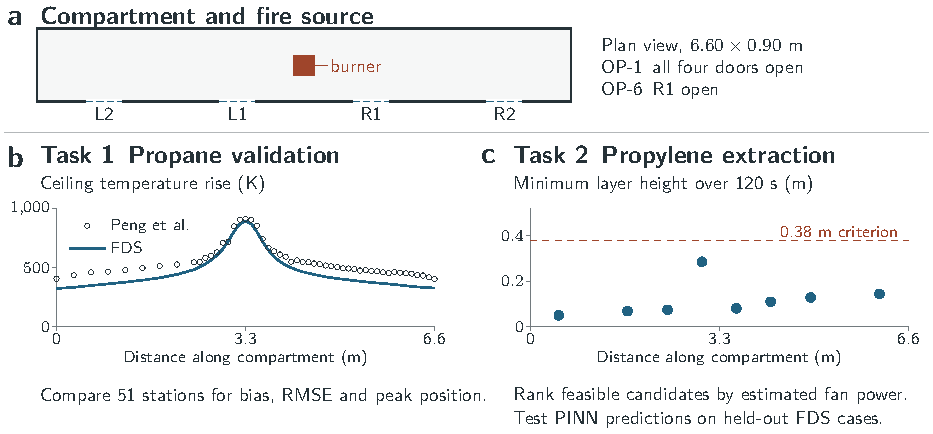
\includegraphics[width=.98\linewidth]{figures/study-workflow.pdf}}{Query order for Bayesian optimisation (BO) and the genetic algorithm (GA, seed 0). Rows increase in curtain depth and columns in flow. Teal marks the largest clearance margin in the archived set.}


\subhead{2.1\quad Task 1 --- Propane fire and ceiling-jet validation}
The geometry follows Fig.~1 of the Topic B brief and the compartment tested by Peng et al.~\cite{peng}. The compartment measured $6.60 \times 0.90 \times 0.76$~m internally, with a 0.25~m square burner on the floor at $x=3.30$~m. Along one side wall, the openings were L2, L1, R1 and R2 in order of increasing $x$. Each was 0.43~m wide and 0.63~m high. The domain extended outside this wall to $y=1.40$~m so that air could enter at one height and leave through the same door at another. The reference ambient temperature was $27.5\,^{\circ}$C.

Group~18 used both nominal fire powers, 47.2 and 106.2~kW, under each door state, OP-1 with all four doors open and OP-6 with only R1 open. FDS specifies heat release per unit burner area. Since the burner edges follow the mesh faces, we checked the resulting burner area on each grid together with the heat release rate recorded during the run.

\clearpage
\subhead{Spatial resolution and physical submodels}
The OP-1 study used $132\times28\times19$, $176\times36\times25$ and $220\times48\times32$ cells over the same domain. Following the FDS User’s Guide~\cite{fdsuser}, the characteristic fire diameter was calculated as
\[
 D^*=\left(\frac{\dot Q}{\rho_\infty c_p T_\infty\sqrt{g}}\right)^{2/5}.
\]
Here $\dot Q$ is the nominal fire power and $g$ is gravitational acceleration. The ambient air properties are density $\rho_\infty$, specific heat $c_p$ and absolute temperature $T_\infty$. Dividing $D^*$ by the longest cell dimension gives a common measure of resolution. The change in the longitudinal temperature profile shows what that resolution means for the result.

\subhead{Task 1 --- Controlled comparisons and experimental measurements}
For OP-1 at 106.2~kW, we first held the coarse grid and radiative fraction (0.29) fixed and changed the subgrid closure from Deardorff to WALE~\cite{fdstech}. Yuen et al.\ also compared closures for compartment fires~\cite{yuen}. We then retained Deardorff and set the radiative fraction to 0.20 and 0.50 in separate runs. A further comparison replaced the adiabatic lining with a conducting board. The experiment supplied the board thickness of 15~mm. The FDS Steckler insulation example supplied proxy values for density (200~kg/m$^3$), conductivity (0.10~W/(m\,K)) and specific heat (1.0~kJ/(kg\,K))~\cite{steckler}. Both wall conditions used the $154\times56\times23$ doorway grid for OP-6 and the original coarse grid for OP-1 at 47.2~kW.

Figure~9 of Peng et al.~\cite{peng} gives the measured ceiling-temperature rise along the compartment. We digitised 51 positions on each profile and paired them with readings from modelled 1~mm thermocouples at $z=0.74$~m. At position $i$, the FDS rise is the mean temperature over 90--120~s, weighted by the actual device intervals, less the model ambient temperature. With $e_i=\Delta T_{\mathrm{FDS},i}-\Delta T_{\mathrm{exp},i}$, the mean bias and root mean square error are
\[
 \mathrm{bias}=\frac{1}{51}\sum_{i=1}^{51}e_i,\qquad
 \mathrm{RMSE}=\sqrt{\frac{1}{51}\sum_{i=1}^{51}e_i^2}.
\]
The distance from the burner to the hottest station gives a separate measure of peak displacement. Over the same interval, the R1 profiles show which part of the door admitted cool air and which part carried hot gas out. The wall and radiation comparisons examine how heat loss also affects the ceiling temperature.

\subhead{Compartment plan and extraction layout}
\begingroup\centering
\setlength{\unitlength}{0.88pt}
\begin{picture}(420,104)
\put(24,28){\framebox(363,49.5){}}
\put(24,76){\line(1,0){363}}
\linethickness{2pt}
\multiput(57.55,77.5)(90.75,0){4}{\line(1,0){23.65}}
\linethickness{0.4pt}
\put(69,85){\makebox(0,0){L2}}
\put(160,85){\makebox(0,0){L1}}
\put(251,85){\makebox(0,0){R1}}
\put(342,85){\makebox(0,0){R2}}
\put(178,28){\line(0,1){49.5}}
\put(233,28){\line(0,1){49.5}}
\put(183.5,30.75){\framebox(22,44){}}
\put(205.5,30.75){\framebox(22,44){}}
\put(198.625,45.875){\dashbox{1.25}(13.75,13.75){}}
\linethickness{2pt}
\put(24,28){\line(0,1){49.5}}
\put(387,28){\line(0,1){49.5}}
\linethickness{0.4pt}
\put(24,18){\line(1,0){363}}
\put(24,15){\line(0,1){6}}
\put(387,15){\line(0,1){6}}
\put(205,8){\makebox(0,0){6.60 m}}
\end{picture}\par
\endgroup
\tablenote{Plan view of the nominal inputs. The long wall carries the four labelled doorways. In the paired-flow design, the heavy end lines mark make-up openings, the two full-width interior lines mark curtains and the adjoining rectangles mark ceiling exhausts. The dashed square marks the floor burner under the exhausts. The end openings, curtains and exhausts apply to Task~2.}


\clearpage
\subhead{2.2\quad Task 2 --- Propylene fire and smoke extraction design}
For the nominal 106.2~kW propylene fire, the baseline soot yield was 0.02~kg/kg of fuel and the CO yield was 0.01~kg/kg. Additional runs raised the soot yield to 0.05 and 0.10~kg/kg while retaining the same CO yield. Each of the three soot yields was tested with OP-1 and OP-6, giving six scenarios with the doors held in position throughout each fire. The original design grid had $132\times28\times19$ cells and adiabatic enclosure surfaces.

\subhead{Candidate screening and design changes}
The archived FDS results support two comparisons of checking order. For the original layout, the next choice was a design. For the revised layout, the choice was which of six scenarios to check first at a given flow. We also examined the effect of changing the flow order.

An initial OP-6 screen at baseline soot yield crossed four curtain depths (0, 0.08, 0.16 and 0.24~m) with four total exhaust flows (0.08, 0.16, 0.24 and 0.32~m$^3$/s). The fixed-order benchmark, Bayesian optimisation (BO)~\cite{bo} and a genetic algorithm (GA)~\cite{ga} began with the same four corner designs. Each query revealed one archived FDS margin. BO and GA used only the margins revealed so far to select their next design. We counted all queries through the first discovery of the largest recorded margin and repeated GA with 20 random seeds.

In the revised layout, replacement air enters at floor level through an opening in each end wall. The inlet height is 0.44~m with OP-1 and 0.48~m with OP-6. Above the burner, two ceiling vents each feed a separate exhaust branch. Transverse curtains at $x=2.8$ and 3.8~m extend 0.24~m below the ceiling on either side of the vents.

\reportfigure{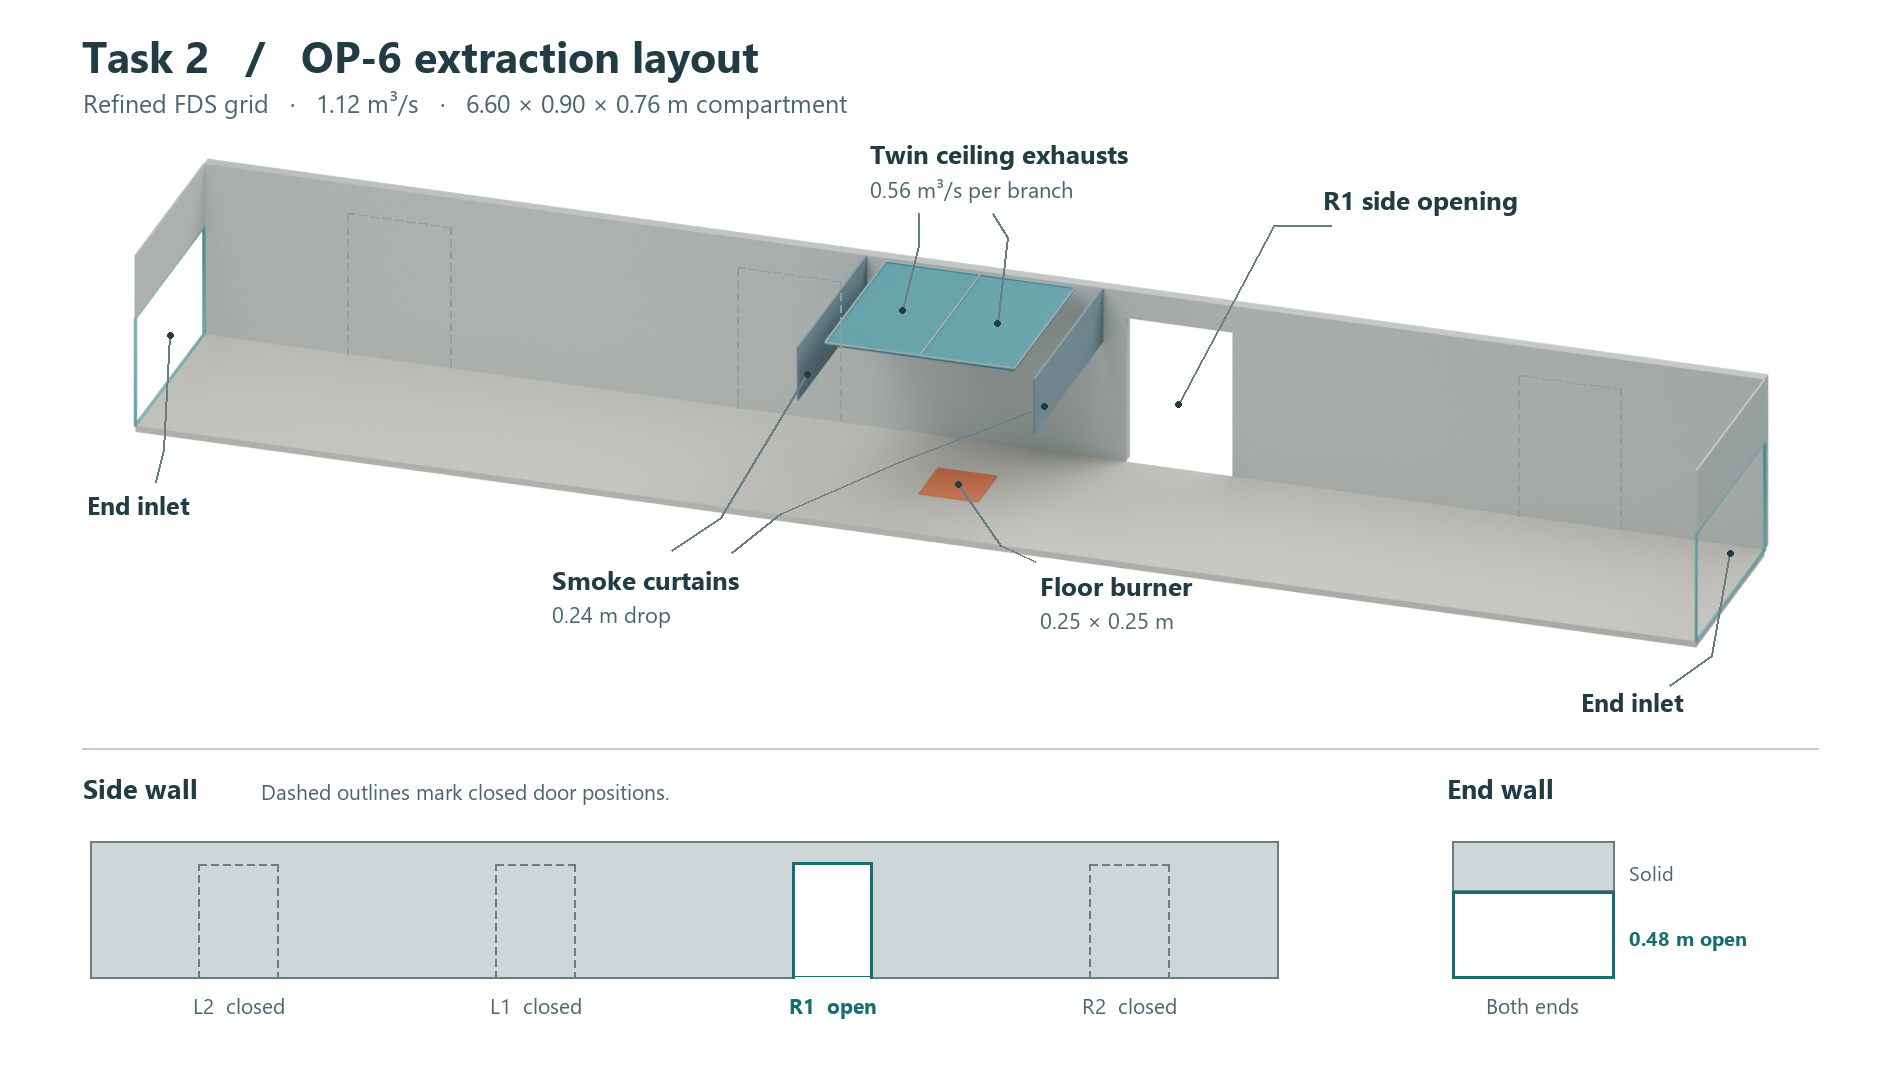
\includegraphics[width=\linewidth]{../figures/op6_1p12_fds_geometry_review.png}}{Cutaway of the refined OP-6 layout. The near wall is omitted from the view. In FDS it is a continuous adiabatic wall at $y=0$. R1 is the only open side door. Dashed outlines mark the three closed door positions. Both end walls admit make-up air through openings extending 0.48~m above the floor.}

With the two branches sharing the flow equally, we compared 0.96 and 1.28~m$^3$/s across all six scenarios. The refined grid also included the intermediate flow of 1.12~m$^3$/s. For the separate ranking study, we excluded both revised inlet families from training and retained increasing power order for the three flows. At each flow the physics-informed neural network (PINN)~\cite{pinn}, direct regression and their equal-weight average ranked the six scenarios from lowest to highest predicted clearance (Section~5.2).

\subhead{Layer-height criterion and local smoke measurements}
FDS reported a thermally inferred layer height $h_j(t)$ along eight vertical columns on the centreplane, $y=0.45$~m. Their longitudinal positions were 0.5, 1.7, 2.4, 3.0, 3.6, 4.2, 4.9 and 6.1~m. Devices were sampled nominally every 0.5~s. For scenario $s$ the sampled margin was
\[
 m_s=\min_{j,\,0\leq t\leq120\,\mathrm{s}} h_{j,s}(t)-0.38\,\mathrm{m}.
\]
Half the compartment height sets the clearance threshold. A single reading below it is sufficient to reject a candidate during screening. A candidate that clears this check needs a full 120~s record for each of the six scenarios. The smallest recorded margin then identifies the door state, soot yield, station and time governing the design. This check covers the eight instrumented columns.

\subhead{Task 2 --- Optical conditions, CO and fan power}
At the same stations, probes at $z=0.38$~m recorded visibility and CO volume fraction. A centreplane map of extinction shows how far smoke extends from the fire. These measurements describe local conditions at half height alongside the temperature-based clearance criterion. Fuel consumption and the specified yield determine the estimated mass of CO generated. The concentration at a probe also depends on how the gas travels, mixes with air and leaves the compartment. Recorded fire power was checked for each comparison.

For a total volume flow $Q$ divided equally between the two short exhaust branches, the estimated electrical input was
\[
 P_{\mathrm{el}}=\frac{Q\,\Delta p}{\eta},\qquad
 \Delta p=\left(f\frac{L}{D_h}+K\right)\frac{\rho}{2}
                 \left(\frac{Q}{2A}\right)^2 .
\]
Each short branch has area $A=0.32$~m$^2$, length $L=0.40$~m and assumed hydraulic diameter $D_h=0.533$~m. The loss calculation takes air density $\rho=1.2$~kg/m$^3$, Darcy friction factor $f=0.02$ and local loss coefficient $K=2$. The two branches run in parallel, so the same pressure drop applies to each. Applying fan efficiency $\eta=0.60$ to the combined flow gives the electrical input for these branches alone.

\subhead{Selection and verification of the design flow}
For the flow selection we doubled the vertical cell count from 19 to 38 and retained the horizontal grid, inlet settings and curtains. The intermediate setting of 1.12~m$^3$/s lies halfway between the original flows. Figure~4b compares all three on the refined grid for OP-6 at baseline soot yield. Table~D3 checks the selected flow against the eight station histories over 120~s for each combination of door state and soot yield.
\clearpage
\subhead{2.3\quad Constrained optimisation of the extraction system}
The brief specifies a minimum clear height and requires a power estimate for mechanical extraction. Group~18 chose minimum required fan input power as the design objective. Let $g$ denote a candidate layout, $Q$ the total extraction rate in m$^3$/s and $P$ the required electrical input in watts. We formulated the design problem as
\begin{equation}
\begin{aligned}
\min_{g,Q,P}\quad &P\\
\mathrm{s.t.}\quad
 &h_{s,i,t}(g,Q)\geq 0.38\,\mathrm{m}
       &&\forall s\in S,\ i\in I,\ t\in T_s,\\
 &P\geq Q\,\Delta p_s(g,Q)/\eta_s(g,Q)
       &&\forall s\in S,\\
 &g\in G,\quad Q\in\mathcal Q(g),\quad P\geq0 .
\end{aligned}
\label{eq:design}
\end{equation}
$G$ contains the candidate vent, curtain and make-up layouts. A door-dependent inlet preset is part of $g$. One setting is specified in advance for each door state and applies to all soot yields in that state. The same $Q$ is selected from the tested flows $\mathcal Q(g)$ for every scenario. The six members of $S$ combine the two door states with the three soot yields. $I$ contains the eight station positions, and $T_s$ contains the stored device times over the full 120~s run. The first constraint tests every recorded station and time. The second sizes electrical input for the largest required power across the scenarios, with pressure drop $\Delta p_s$ in Pa and total efficiency $0<\eta_s\leq1$.

For the two equal-flow branches, we evaluate power using the short-branch loss estimate in Section~2.2. Remaining ductwork and equipment losses are unknown. We evaluate feasibility by enumerating the tested candidates and computing the worst sampled clearance,
\[
m(g,Q)=\min_{s\in S,\ i\in I,\ t\in T_s}
           \{h_{s,i,t}(g,Q)-0.38\,\mathrm{m}\}.
\]
One negative margin excludes a design. A feasible design must have $m\geq0$ over the full set of records, after which its electrical input can be compared with that of other feasible designs. If every candidate falls short, the design with the largest margin provides a starting point for the next layout. The Bayesian and genetic searches in Section~5.2 are assessed on how soon they locate that design.

\clearpage
\reportheading{3.\quad Task 1 --- Ceiling-jet validation and doorway effects}
\subhead{3.1\quad Agreement with the measured temperature profiles}
At 47.2~kW, the coarse-grid OP-1 profile underestimated the measured temperature rise by 192~K on average. With only R1 open, the signed error averaged +6~K but the RMSE remained 33~K. At 106.2~kW the largest discrepancy occurred under OP-6. The adiabatic calculation placed the hottest station 0.80~m left of the burner. The experiment placed it 0.20~m left. The model captured the direction of displacement and exaggerated its magnitude.
\newcommand{\validationpanel}[3]{%
\begin{tikzpicture}
\begin{axis}[width=.475\linewidth,height=3.9cm,xmin=-340,xmax=340,ymin=0,ymax=1350,
xtick={-300,0,300},ytick={0,600,1200},axis lines=left,ymajorgrids,grid style={gray!14},
tick align=outside,title={#2\quad #3 kW},title style={font=\sffamily\small\bfseries,color=ink,at={(.5,.97)}},
tick label style={font=\sffamily\scriptsize},enlarge x limits=false]
\addplot[teal,thick,no marks] table[col sep=comma,x expr=\thisrow{model_x_cm}-330,y=fds_rise_K]{../../05_Calculations/#1_90_120.csv};
\addplot[only marks,mark=o,mark size=1.2pt,rust] table[col sep=comma,x=figure_r_cm,y=exp_rise_K]{../../05_Calculations/#1_90_120.csv};
\end{axis}\end{tikzpicture}}
\reportfigure{{\sffamily\small Temperature rise (K)\hfill
\textcolor{teal}{\rule[.4ex]{14pt}{1.1pt}} FDS\quad
\textcolor{rust}{$\circ$} Peng et al.\par}
\begin{tabular}{@{}cc@{}}
\validationpanel{op1_47_coarse}{OP-1}{47.2}&\validationpanel{op1_106_coarse}{OP-1}{106.2}\\
\validationpanel{op6_47_coarse}{OP-6}{47.2}&\validationpanel{op6_106_coarse}{OP-6}{106.2}
\end{tabular}\par{\sffamily\small Distance from the fire axis (cm)}}{Figure 1. Measured and simulated ceiling temperature rise. Each panel uses the same axes. The experimental markers are digitised from Peng et al.\ (2021), Fig.~9. The lines show coarse-grid FDS averages over 90--120~s.}

Peng et al.\ reported stable-phase temperatures and illustrated repeatability with OP-1 at 70.8~kW (their Fig.~2). Their reported relative uncertainty of up to 8\% concerns measured temperature. For the four coarse-grid comparisons, we checked the sensitivity to time averaging by comparing 90--105~s with 105--120~s at each station. The largest absolute change at any station ranged from 9.2 to 28.2~K across the four cases. The small signed mean error for OP-6 at low power should therefore be read alongside its spatial RMSE and the choice of averaging window.
\subhead{3.2\quad Sensitivity to grid and model inputs}
For OP-1, coarse, medium and fine grids gave RMSEs of 192.4, 187.7 and 176.2~K at low power, and 82.0, 75.7 and 79.9~K at high power. The high-power error reached its minimum on the medium mesh. Grid refinement alone therefore offers limited grounds for selecting the fine-grid solution. On the high-power coarse grid, switching from Deardorff to WALE reduced RMSE from 82.0 to 77.0~K. Holding Deardorff fixed and changing the radiative fraction from 0.29 to 0.20 or 0.50 gave 74.6 or 131.1~K. Radiative partitioning influenced the temperature prediction more strongly than the tested change of closure in this case.

\clearpage
\subhead{3.3\quad Door exchange and enclosure heat loss}
At 106.2~kW total doorway inflow fell from 0.318~kg/s in OP-1 to 0.095~kg/s in OP-6. At R1, velocity changed from inward to outward between 0.30 and 0.38~m in OP-1 and between 0.22 and 0.30~m in OP-6 (Figure~B1). At 47.2~kW the outward stream at 0.38~m was hotter in OP-6 (212.1 versus 64.8$\,^{\circ}$C). Air entering from R1 could deflect the plume towards the closed side, consistent with the observed peak displacement. The probes establish the doorway exchange; plume deflection is inferred.

For OP-6 at 106.2~kW, the 15~mm proxy board reduced profile RMSE from 361.4 to 100.7~K on the matched diagnostic grid. Peak-position error fell from 0.70 to 0.10~m. The 24 stations from 1.0 to 3.3~m on the R1 side still averaged 112.5~K below the measurements (Figure~2 and Table~F1). Over 90--120~s the board run gave signed domain radiative, convective and conductive terms of $-61.4$, $-34.2$ and $-9.6$~kW, including the exterior extension.
\reportfigure{\begin{tikzpicture}
\begin{axis}[width=.94\linewidth,height=5.7cm,xmin=-340,xmax=340,ymin=0,ymax=1350,ytick={0,300,600,900,1200},xtick={-300,-150,0,150,300},
xlabel={Distance from the fire axis (cm)},ylabel={Temperature rise (K)},axis lines=left,ymajorgrids,grid style={gray!15},
legend columns=3,legend style={at={(.5,1.03)},anchor=south,draw=none,/tikz/every even column/.append style={column sep=6pt}}]
\addplot[gray,thick,dashed] table[col sep=comma,x expr=\thisrow{model_x_cm}-330,y=fds_rise_K]{../../05_Calculations/op6_106_doorflow_90_120.csv};
\addlegendentry{Adiabatic}
\addplot[teal,thick] table[col sep=comma,x expr=\thisrow{model_x_cm}-330,y=fds_rise_K]{../../05_Calculations/op6_106_board_doorflow_90_120.csv};
\addlegendentry{Conducting board}
\addplot[only marks,rust,mark=o,mark size=1.6pt] table[col sep=comma,x=figure_r_cm,y=exp_rise_K]{../../05_Calculations/op6_106_board_doorflow_90_120.csv};
\addlegendentry{Peng et al.}
\end{axis}\end{tikzpicture}}{Figure 2. OP-6 at 106.2 kW. The adiabatic and conducting-board predictions share the doorway diagnostic grid. The measured and simulated profiles use the same coordinate origin as Figure 1.}

On the 47.2~kW OP-1 coarse grid, the same board increased RMSE from 192.4 to 243.3~K. The peak remained over the burner, but its rise fell from 435 to 340~K against a measured 580~K. In the adiabatic OP-1 diagnostic, the 51-station mean cold bias was 191.8~K for the thermocouples and 187.1~K for the co-located gas. The simulated sensor response accounts for only 4.7~K of that difference (Figure~F1). Doorway sensitivity motivated testing both door states and the far ends in Task~2. The propane benchmark assesses ceiling temperature. The propylene clearance margins come from FDS with the prescribed adiabatic enclosure and extraction settings.

\clearpage
\reportheading{4.\quad Task 2 --- Smoke extraction design and optimisation}
\subhead{4.1\quad FDS screening of the original 16 designs}
The best of the 16 original OP-6 designs combined a 0.16~m curtain with 0.32~m$^3$/s extraction at baseline soot yield (Appendix~C). Even this design gave a minimum interface of 0.095~m, leaving a deficit of 0.285~m against the 0.38~m target. The next trials therefore changed where replacement air entered and where the ceiling vents collected smoke.

\subhead{4.2\quad Locating the failure and adapting the inlets}
An OP-6 trial used 0.36~m end inlets, 0.24~m curtains and 1.28~m$^3$/s total extraction. At soot yield 0.05 the far-end column ($x=6.1$~m) recorded an interface of 0.353~m at 83.0~s. The readings immediately before and after both exceeded 0.60~m. The low reading counts as a breach of the thermal criterion. At the same point visibility at half height remained 30~m and the vertical temperature gradient was weak, leaving the extent of smoke there uncertain.

The choice of inlet height for OP-6 can be seen by comparing the two inlet heights at each of two soot yields on the original grid. At 1.28~m$^3$/s, raising the end openings from 0.44 to 0.48~m increased the minimum interface from 0.431 to 0.583~m at yield 0.02, but reduced it from 0.524 to 0.497~m at yield 0.05. Taking the lower reading for each inlet height, the taller opening raised the limiting value from 0.431 to 0.497~m. We therefore used 0.48~m for OP-6 in the six-scenario check, with 0.44~m for OP-1 and 0.24~m curtains in both states.
\reportfigure{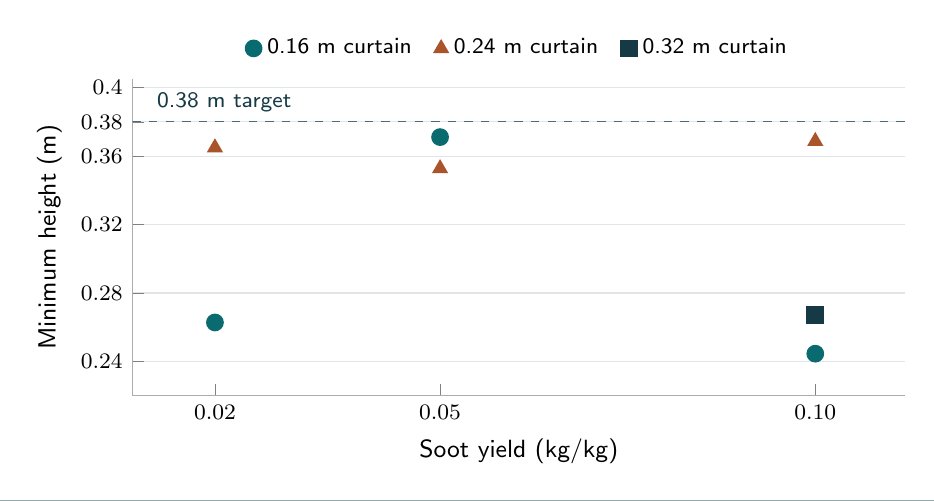
\begin{tikzpicture}
\begin{axis}[width=.94\linewidth,height=5.6cm,xmin=.009,xmax=.112,ymin=.22,ymax=.405,
xtick={.02,.05,.10},ytick={.24,.28,.32,.36,.38,.40},scaled ticks=false,
xticklabel style={/pgf/number format/fixed,/pgf/number format/fixed zerofill,/pgf/number format/precision=2},
yticklabel style={/pgf/number format/fixed},axis lines*=left,ymajorgrids,grid style={ink!13},
xlabel={Soot yield (kg/kg)},ylabel={Minimum height (m)},legend columns=3,legend style={at={(.5,1.03)},anchor=south,draw=none,/tikz/every even column/.append style={column sep=6pt}}]
\addplot[only marks,teal,mark=*,mark size=3pt] coordinates {(0.02,0.2627491) (0.05,0.37114426) (0.1,0.24450079)};\addlegendentry{0.16 m curtain}
\addplot[only marks,rust,mark=triangle*,mark size=3pt] coordinates {(0.02,0.36496348) (0.05,0.3527722) (0.1,0.36869806)};\addlegendentry{0.24 m curtain}
\addplot[only marks,ink,mark=square*,mark size=3pt] coordinates {(0.10,0.26696128)};\addlegendentry{0.32 m curtain}
\addplot[ink!75,dashed,forget plot] coordinates {(.009,.38) (.112,.38)};
\node[anchor=south west,font=\sffamily\footnotesize,text=ink] at (axis cs:.011,.38){0.38 m target};
\end{axis}\end{tikzpicture}}{Figure 3. Minimum thermal layer height for the seven completed OP-6 curtain trials at 1.28 m$^3$/s. Each marker represents eight stations over 120 s. The 0.32 m curtain was evaluated at soot yield 0.10 kg/kg.}

\clearpage
\subhead{4.3\quad Selecting the design flow}
With two ceiling vents, 0.24~m curtains and the inlet height set for each door state, the remaining choice was the common extraction rate. We tested 1.12~m$^3$/s, halfway between the original settings of 0.96 and 1.28~m$^3$/s, to see whether it could maintain the interface above half height under both door states at all three soot yields.
\reportfigure{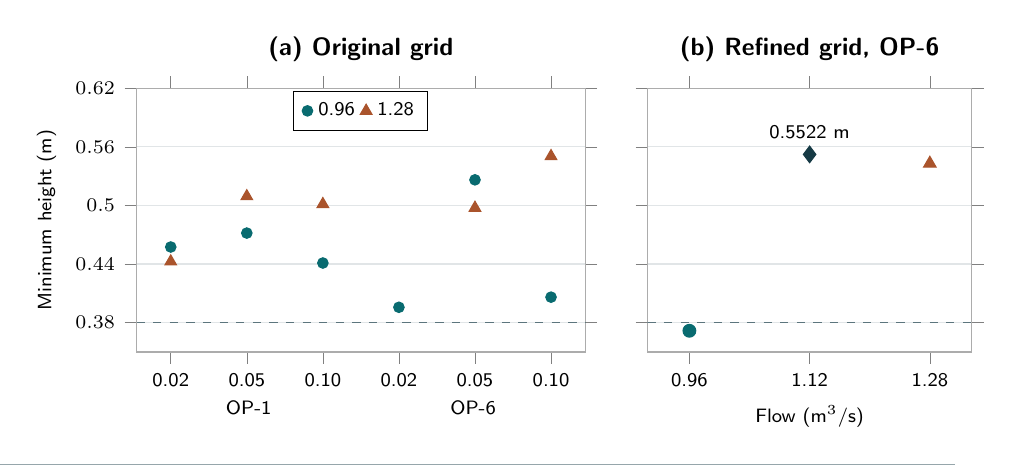
\begin{tikzpicture}
\pgfplotsset{flowpanel/.style={
 scale only axis,height=3.35cm,ymin=.35,ymax=.62,ytick={.38,.44,.50,.56,.62},
 scaled ticks=false,yticklabel style={/pgf/number format/fixed,/pgf/number format/precision=2},
 ymajorgrids,grid style={ink!13},tick align=outside,title style={font=\sffamily\small\bfseries},
 tick label style={font=\sffamily\scriptsize},label style={font=\sffamily\scriptsize}}}
\begin{axis}[flowpanel,name=original,width=.47\linewidth,xmin=.55,xmax=6.45,
 title={(a) Original grid},ylabel={Minimum height (m)},
 xtick={1,2,3,4,5,6},xticklabels={0.02,0.05,0.10,0.02,0.05,0.10},
 clip=false,legend style={at={(.50,.99)},anchor=north,font=\sffamily\scriptsize,fill=white},
 legend columns=2]
\addplot[only marks,mark=*,teal,mark size=1.9pt] coordinates {(1,.45742963) (2,.47169434) (3,.44104958) (4,.39573017) (5,.52617570) (6,.40609647)};
\addlegendentry{0.96}
\addplot[only marks,mark=triangle*,rust,mark size=2.4pt] coordinates {(1,.44252295) (2,.50930185) (3,.50127480) (4,.58267633) (5,.49747471) (6,.55033156)};
\addlegendentry{1.28}
\addplot[ink!70,dashed] coordinates {(.55,.38)(6.45,.38)};
\node[anchor=north,font=\sffamily\scriptsize] at (axis description cs:.25,-.15) {OP-1};
\node[anchor=north,font=\sffamily\scriptsize] at (axis description cs:.75,-.15) {OP-6};
\end{axis}
\begin{axis}[flowpanel,at={(original.east)},anchor=west,xshift=.065\linewidth,
 width=.34\linewidth,xmin=.65,xmax=3.35,title={(b) Refined grid, OP-6},
 xtick={1,2,3},xticklabels={0.96,1.12,1.28},xlabel={Flow (m$^3$/s)},yticklabels=\empty]
\addplot[ink!70,dashed] coordinates {(.65,.38)(3.35,.38)};
\addplot[only marks,mark=*,teal,mark size=2.3pt] coordinates {(1,.37169)};
\addplot[only marks,mark=diamond*,ink,mark size=3pt] coordinates {(2,.5522)};
\addplot[only marks,mark=triangle*,rust,mark size=2.6pt] coordinates {(3,.5429)};
\node[anchor=south,font=\sffamily\scriptsize] at (axis cs:2,.558) {0.5522 m};
\end{axis}
\end{tikzpicture}}{Figure 4. The dashed line marks the 0.38~m thermal-interface target. (a) Two reference flows (m$^3$/s) on the original grid, grouped by door state and soot yield (kg/kg). (b) Three flows on the same refined grid for OP-6 at yield 0.02. The 1.12 and 1.28~m$^3$/s minima cover 120~s. The 0.96~m$^3$/s record ends at 98~s. Figure~5 gives the six-scenario check at 1.12~m$^3$/s.}


Baseline soot gave the smallest original-grid margin at both reference flows (Figure~4a). At 0.96~m$^3$/s, only 15.7~mm separated the lowest interface from the target, within one 40~mm vertical cell. When the cell height was halved, the far-end column in the OP-6 baseline case reached 0.3717~m at 98.0~s and screening stopped (Table~D2). Figure~4b compares the three flows at this finer spacing.

\subhead{Clearance and power at 1.12~m$^3$/s}
For OP-6 at baseline soot yield, the lowest interface over 120~s was 0.5522~m at 1.12~m$^3$/s and 0.5429~m at 1.28~m$^3$/s. At the proposed setting each branch carries 0.56~m$^3$/s, giving a velocity of 1.75~m/s and an estimated pressure drop of 3.70~Pa. At the assumed fan efficiency of 0.60, the two branches together require 6.91~W. This is about 33\% below the 10.32~W at 1.28~m$^3$/s, so we carried 1.12~m$^3$/s into the six-scenario check.

\clearpage
\subhead{Six-scenario FDS confirmation}
In all six refined-grid runs at 1.12~m$^3$/s, the interface stayed above 0.38~m at each of the eight stations for the full 120~s (Table~D3). Mean heat release over 90--120~s was 102.1--103.9~kW against the nominal 106.2~kW. The far-end column governed clearance. In OP-6 at soot yield 0.05, it recorded 0.4358~m at $x=6.1$~m and 113.0~s, leaving 55.8~mm above the target. There the longitudinal velocity changed sign between $z=0.42$ and 0.44~m. Figure~A2 shows smoke at half height at the same time.
% Rows are the six refined-grid FDS station minima at 1.12 m3/s.
% PINN points are the forecasts frozen in hybrid_frozen_1p12.json.
\reportfigure{\begin{tikzpicture}
\begin{axis}[width=.96\linewidth,height=5.1cm,xmin=.55,xmax=6.45,
 ymin=.355,ymax=.61,xtick={1,2,3,4,5,6},
 xticklabels={{OP-1\\0.02},{OP-1\\0.05},{OP-1\\0.10},{OP-6\\0.02},{OP-6\\0.05},{OP-6\\0.10}},
 xticklabel style={align=center},ytick={.38,.44,.50,.56,.60},ylabel={Minimum height (m)},
 ymajorgrids,unbounded coords=discard,
 legend style={at={(.5,1.03)},anchor=south,legend columns=3,draw=none},
 /tikz/every even column/.append style={column sep=5pt}]
\addplot[only marks,mark=*,teal,mark size=2.7pt]
 table[col sep=comma,x=position,y=fds_m]{data/verified-flow-forecast.csv};
\addlegendentry{Refined-grid FDS}
\addplot[only marks,mark=diamond*,rust,mark options={fill=white},mark size=3.2pt]
 table[col sep=comma,x expr=\thisrow{position}+.10,y=pinn_m]{data/verified-flow-forecast.csv};
\addlegendentry{Frozen PINN}
\addplot[ink,densely dashed] coordinates {(.55,.38)(6.45,.38)};
\addlegendentry{Height target}
\draw[teal,thin] (axis cs:5,.385)--(axis cs:5,.430);
\node[anchor=west,font=\sffamily\scriptsize,text=teal] at (axis cs:5.04,.408) {55.8 mm};
\end{axis}\end{tikzpicture}}{Figure 5. Refined-grid verification at 1.12~m$^3$/s by door state and soot yield (kg/kg). Filled circles are the FDS minima over eight stations and 120~s. Open diamonds show the three PINN forecasts frozen before the corresponding runs.}


\subhead{4.4\quad CO generation and local smoke conditions}
Each kilogram of fuel consumed produces 10~g of CO at the specified yield. In earlier OP-6 trials with 0.24~m curtains and 1.28~m$^3$/s extraction, integrated fire power gave estimated CO masses of 2.76, 2.81 and 2.94~g as soot yield rose. Peak half-height concentrations were 20.0, 26.2 and 163.5~ppm. Capture near the plume and a clear make-up air path help remove CO. In the original OP-6 layout with baseline soot and 0.16~m curtains, increasing extraction from 0.16 to 0.64~m$^3$/s reduced mean far-end CO from 101.04 to 0.62~ppm. Table~1 gives local exposure for the recommended layout.

\tabletitle{Table 1. Half-height exposure indicators at the selected 1.12 m$^3$/s setting. Each value is the extreme over eight probes and 120 s on the refined grid.}
\begin{reporttable}{L{.18}L{.24}L{.31}L{.27}}
\rowcolor{tablegrey}Door&Soot (kg/kg)&Min. visibility (m)&Max. CO (ppm)\\
OP-1&0.02&30.00&0.65\\
OP-1&0.05&30.00&0.26\\
OP-1&0.10&30.00&0.28\\
OP-6&0.02&24.15&7.59\\
OP-6&0.05&16.42&11.81\\
OP-6&0.10&4.06&32.83\\
\end{reporttable}
In OP-6 at yield 0.10, the probe near the burner ($x=3.6$~m) recorded both peak CO and minimum visibility at 3.0~s. The thermal minimum occurred much later and farther away, at $x=6.1$~m and 113.0~s in OP-6 at yield 0.05.

\clearpage
\reportheading{5.\quad BO, GA and PINN in the joint design}
\subhead{5.1\quad Minimum-height predictions and FDS verification}
A brief fall below 0.38~m at any of the eight stations is enough to breach the 120~s design criterion. We therefore compared forecasts using the lowest FDS reading in each run (time-series errors are in Appendix~D). In the first 20 runs on the 19-cell vertical grid, correcting each station minimum reduced the mean absolute error (MAE) in the compartment minimum from 27.03 to 8.26~cm. The larger sample included 27 completed runs for 26 designs across OP-1 and OP-6. Each design and its mesh variants were held out together. MAE was 6.97~cm for the corrected PINN, 7.39~cm for direct regression and 6.70~cm for their equal-weight average. Of the eight actual breaches the models missed seven, four and four, respectively. Among the 19 passing runs, the same models raised zero, one and zero false alarms. Table~E2 extends the comparison to whole inlet-layout families.

The open diamonds in Figure~5 show predictions made before the FDS results were available. For OP-1 at soot yields 0.05 and 0.10, the PINN underestimated minimum height by 5.1 and 34.8~mm. The hybrid underestimated it by 1.7 and 5.2~cm. The error changed direction in the case governing the selected 1.12~m$^3$/s flow. For OP-6 at yield 0.05, the PINN gave 0.5766~m and the hybrid 0.5576~m, overpredicting the FDS minimum by 140.8 and 121.8~mm. From the six refined-grid runs the lowest recorded height was 0.4358~m, giving the design margin of 55.8~mm (Table~C3).

\subhead{5.2\quad Searching joint flow and curtain-depth candidates}
Both replays started at the same four corner designs. BO updated a Gaussian process with revealed FDS margins and used the chance of clearing the height target and potential flow savings to choose the next query. GA encoded flow and curtain depth as integer genes and used predicted feasibility and flow to select, cross and mutate candidates.

The fixed order found the largest recorded margin on query 16, BO on query 7 and GA on queries 6--11 across 20 seeds. Every tested design breached the target. For a larger search, the proposed loop uses the PINN for a clearance prior, BO to score the next query, GA to search the acquisition function and FDS to update the model. The replays benchmark BO and GA separately.

\subhead{5.3\quad PINN prioritisation for the revised layout}

At fixed ascending flow, checking OP-6 at the lowest soot yield first exposed the breach at 0.96~m$^3$/s, and six further checks confirmed 1.12~m$^3$/s. Ordering scenarios by predicted lowest height took 7--11 checks with PINN, seven with direct regression and 7--9 with their average.

Allowing the forecasts to reorder flows as well, PINN took 7--17 refined-grid checks to find a passing flow and 9--17 to establish the lowest-power tested choice. The fixed order and direct regression took seven for both, and the hybrid took 7--9. On the original grid all methods took six for both. The ranges allow either outcome for unarchived cases.

\clearpage
\reportheading{6.\quad Conclusions and design recommendation}
The single open doorway concentrated exchange at R1. The measured ceiling-temperature peak shifted towards the closed side. Wall heat transfer improved the high-power OP-6 prediction but deepened the low-power OP-1 cold bias. Agreement in peak position alone therefore gives an incomplete picture of temperature accuracy.

For the propylene design, we recommend 1.12~m$^3$/s with two ceiling exhausts, 0.24~m curtains and end openings preset to 0.44~m for OP-1 or 0.48~m for OP-6. This was the lowest-power feasible choice among the three tested flows. The 0.96~m$^3$/s setting breached the height constraint under refinement. At 1.12~m$^3$/s, the smallest of the six refined-grid margins was 55.8~mm, at $x=6.1$~m and 113.0~s under OP-6 at soot yield 0.05. Estimated short-branch power fell from 10.32~W at 1.28~m$^3$/s to 6.91~W. Fan selection would also require full-system losses and a fan curve.

In the original layout, BO and GA found the least severe breach earlier in a replay of 16 designs. In the revised layout, a separate replay ranked the six scenarios within each flow. Checking OP-6 at baseline soot first already gave the fewest possible checks in this comparison. Using BO or GA to choose a design and then using the PINN to schedule its FDS runs remains a proposed workflow.

\bigskip\reportheading{References}
The Hong Kong Polytechnic University. \textit{BSE3322 Mini-design Project: CFD Fire Simulation Study, Topic B.} Project brief, Fig.~1 and Table~1, pp.~1--3.

Peng, M., Cheng, X., Cong, W., Yang, H., Shahid, M.~U., Yuen, R., and Zhang, H. (2021). Experimental study on temperature profile in long-narrow compartment fire with multiple lateral openings. \textit{Tunnelling and Underground Space Technology}, 117, 104018.

Yuen, A.~C.~Y., Yeoh, G.~H., Timchenko, V., and Barber, T. (2015). LES and multi-step chemical reaction in compartment fires. \textit{Numerical Heat Transfer, Part A: Applications}, 68(7), 711--736. \url{https://doi.org/10.1080/10407782.2015.1012886}

McGrattan, K., Hostikka, S., Floyd, J., McDermott, R., Vanella, M., Mueller, E., and Paul, C. (2025). \textit{Fire Dynamics Simulator User's Guide}, sixth edition, revision FDS 6.10.1. NIST Special Publication 1019. \url{https://doi.org/10.6028/NIST.SP.1019}

\clearpage
\reportheading{Appendix A.\quad Case register}
Propane results use FDS 6.10.1 and time-weighted means over 90--120~s. The four assigned base combinations comprise OP-1 and OP-6 at 47.2 and 106.2~kW. Reading the ordered HRRs in Peng et al., Table~2, gives Tests 4, 8, 44 and 48, respectively (low then high power within each door state). Successful FDS runs number 4, 9, 2 and 5 for these conditions, including grid, wall, model and diagnostic variants. The assignment table specifies eight cases but identifies only these four distinct even-group conditions. Propylene screening records extend to the first observed rejection or 120~s. The original-grid paired-flow comparison covers eight stations over 120~s; the refined 0.96~m$^3$/s OP-6 case stopped at its first recorded breach.
\subhead{Appendix B.\quad Grid and door-flow comparisons}
The characteristic fire diameters were 0.283 and 0.391~m at 47.2 and 106.2~kW. Their ratios to the longest cell dimensions were 5.65/7.82, 7.27/10.05 and 9.42/13.03 on the coarse, medium and fine meshes. Corresponding snapped burner areas were 0.06250, 0.06125 and 0.06300~m$^2$.
\tabletitle{B1. Doorway diagnostic cases, 90--120 s.}
\begin{reporttable}{L{.18}L{.20}L{.21}L{.21}L{.20}}
\rowcolor{tablegrey}Door&Fire (kW)&In (kg/s)&Out (kg/s)&RMSE (K)\\
OP-1&47.2&0.260&0.261&166.6\\
OP-1&106.2&0.318&0.322&55.0\\
OP-6&47.2&0.094&0.096&61.4\\
OP-6&106.2&0.095&0.098&361.4\\
\end{reporttable}
\reportfigure{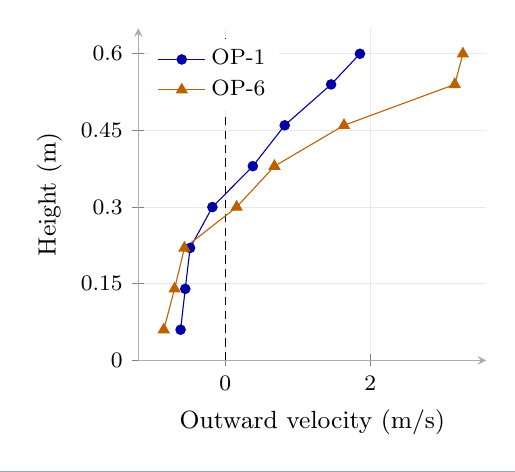
\begin{tikzpicture}
\begin{axis}[width=.495\linewidth,height=5.8cm,axis lines=left,ymin=0,ymax=.65,
ytick={0,.15,.30,.45,.60},xmin=-1.2,xmax=3.6,
xlabel={Outward velocity (m/s)},ylabel={Height (m)},grid=major,grid style={gray!18},
tick label style={font=\footnotesize},label style={font=\small},
legend style={at={(.03,.97)},anchor=north west,font=\footnotesize,draw=none}]
\addplot[black,densely dashed,forget plot] coordinates {(0,0) (0,.63)};
\addplot[blue!65!black,mark=*,mark size=1.7pt] coordinates {(-0.6169,0.06) (-0.5525,0.14) (-0.4858,0.22) (-0.1781,0.3) (0.3791,0.38) (0.8191,0.46) (1.459,0.54) (1.8563,0.6)};
\addlegendentry{OP-1}
\addplot[orange!75!black,mark=triangle*,mark size=2.2pt] coordinates {(-0.8488,0.06) (-0.6996,0.14) (-0.5641,0.22) (0.1562,0.3) (0.6777,0.38) (1.6367,0.46) (3.164,0.54) (3.2764,0.6)};
\addlegendentry{OP-6}
\end{axis}\end{tikzpicture}%
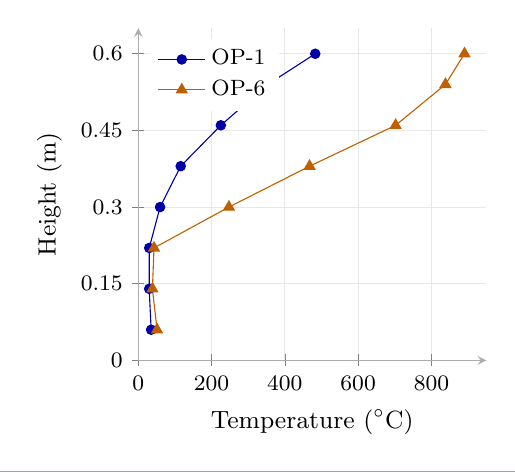
\begin{tikzpicture}
\begin{axis}[width=.495\linewidth,height=5.8cm,axis lines=left,ymin=0,ymax=.65,
ytick={0,.15,.30,.45,.60},xmin=0,xmax=950,
xlabel={Temperature ($^\circ$C)},ylabel={Height (m)},grid=major,grid style={gray!18},
tick label style={font=\footnotesize},label style={font=\small},
legend style={at={(.03,.97)},anchor=north west,font=\footnotesize,draw=none}]

\addplot[blue!65!black,mark=*,mark size=1.7pt] coordinates {(35.0545,0.06) (29.7306,0.14) (29.8055,0.22) (59.4344,0.3) (115.7244,0.38) (225.2291,0.46) (353.3391,0.54) (482.9451,0.6)};
\addlegendentry{OP-1}
\addplot[orange!75!black,mark=triangle*,mark size=2.2pt] coordinates {(51.0932,0.06) (38.5634,0.14) (42.8348,0.22) (247.3595,0.3) (467.4785,0.38) (702.2993,0.46) (838.2762,0.54) (890.311,0.6)};
\addlegendentry{OP-6}
\end{axis}\end{tikzpicture}}{Figure B1. R1 doorway profiles at eight elevations for the adiabatic 106.2~kW diagnostic runs. Each point is a 90--120~s average. Negative velocity denotes incoming air.}

\clearpage
\reportheading{Appendix C.\quad Original OP-6 search}
\tabletitle{C1. Sampled height margin (mm) as a function of curtain depth and flow.}
\begin{reporttable}{L{.28}L{.18}L{.18}L{.18}L{.18}}
\rowcolor{tablegrey}Curtain depth&\multicolumn{4}{c}{Total flow (m$^3$/s)}\\
(m)&0.08&0.16&0.24&0.32\\
0.00&$-334$&$-331$&$-295$&$-289$\\
0.08&$-336$&$-331$&$-288$&$-294$\\
0.16&$-335$&$-331$&$-296$&$-285$\\
0.24&$-336$&$-337$&$-294$&$-302$\\
\end{reporttable}
\clearpage
\reportheading{Appendix D.\quad Paired-flow data coverage}
\tabletitle{Table D1. Minimum thermal interface height (m) across eight stations, 0--120~s, original grid. The target is 0.380~m.}
\begin{reporttable}{L{.23}L{.23}L{.27}L{.27}}
\rowcolor{tablegrey}Door state&Soot (kg/kg)&0.96 m$^3$/s&1.28 m$^3$/s\\
OP-1&0.02&0.4574&\textbf{0.4425}\\
OP-1&0.05&0.4717&0.5093\\
OP-1&0.10&0.4410&0.5013\\
OP-6&0.02&\textbf{0.3957}&0.5827\\
OP-6&0.05&0.5262&0.4975\\
OP-6&0.10&0.4061&0.5503\\
\end{reporttable}
The 1.28~m$^3$/s minima in Table D1 were checked against the raw device histories and successful completion logs. At 0.96~m$^3$/s the archived per-station reductions cover eight stations and 0--120~s in each of the six cases. Some local raw folders contain earlier, interrupted runs. The low-flow comparisons use the archived full-duration station data.

\tabletitle{Table D2. Revised layout, OP-6, soot yield 0.02, 38-cell vertical grid. The minimum is taken over all eight stations in the recorded interval.}
\begin{reporttable}{L{.20}L{.22}L{.21}L{.37}}
\rowcolor{tablegrey}$Q$ (m$^3$/s)&Fan input (W)&Minimum (m)&FDS record\\
0.96&4.35&0.3717&Breach at 98.0 s\\
1.12&6.91&0.5522&Complete, 120 s\\
1.28&10.32&0.5429&Complete, 120 s\\
\end{reporttable}

Combined fan input uses the two short branches and efficiency of 0.60 in Section~2.2. The 1.12~m$^3$/s case minimises power in Table D2. Table D3 distinguishes cases that reached 120~s from those still accumulating device records. A recorded height below 0.38~m establishes a breach even before 120~s.
\tabletitle{Table D3. Refined-grid evidence at 1.12~m$^3$/s. Partial minima cover only the recorded interval.}
\begin{reporttable}{L{.16}L{.18}L{.21}L{.22}L{.23}}
\rowcolor{tablegrey}Door&Soot (kg/kg)&Status&Record (s)&Minimum (m)\\
\csname @@input\endcsname sections/intermediate-coverage.tex
\end{reporttable}
\clearpage
\reportheading{Appendix E.\quad Surrogate event scoring}
The physics-informed extreme learning machine used 96 fixed tanh units and a least-squares output fit with ridge coefficient 0.1. A simplified upper-layer volume balance constrained the weighted mean layer thickness under an assumption of lateral uniformity. A short event was a continuous excursion below 0.38~m at one station lasting at most 2~s. An event counted as a match when the intersection of the predicted and observed intervals covered at least half their union, with one-to-one matching. Linear interpolation between device records approximately 0.5~s apart limits the precision of short event durations.
\subhead{Testing the minimum-height decision directly}
On the earlier 20-case, 19-cell vertical grid cohort, whole-design holdout error in minimum height fell from 27.03 to 8.26~cm after fitting a station-minimum correction. Missed breaches fell from eight to six of eight, with one false alarm among twelve passing runs. Section~5 gives the expanded comparison.

For the refined OP-6 low-flow case, the corrected forecast frozen before completion was 0.4710~m. The 0.3717~m breach at 98~s gives an overprediction of at least 9.9~cm because the run stopped early. At 1.12~m$^3$/s, forecasts issued at 60 and 90~s identified the limiting station at $x=4.2$~m after its minimum at 49.50~s.

A separate two-second warning test used observations from running simulations. At a retrospectively matched count of 33 false alarms, local-height and multistation-temperature models detected the same four of 25 short events, with a mean lead of 0.73~s.

\reportfigure{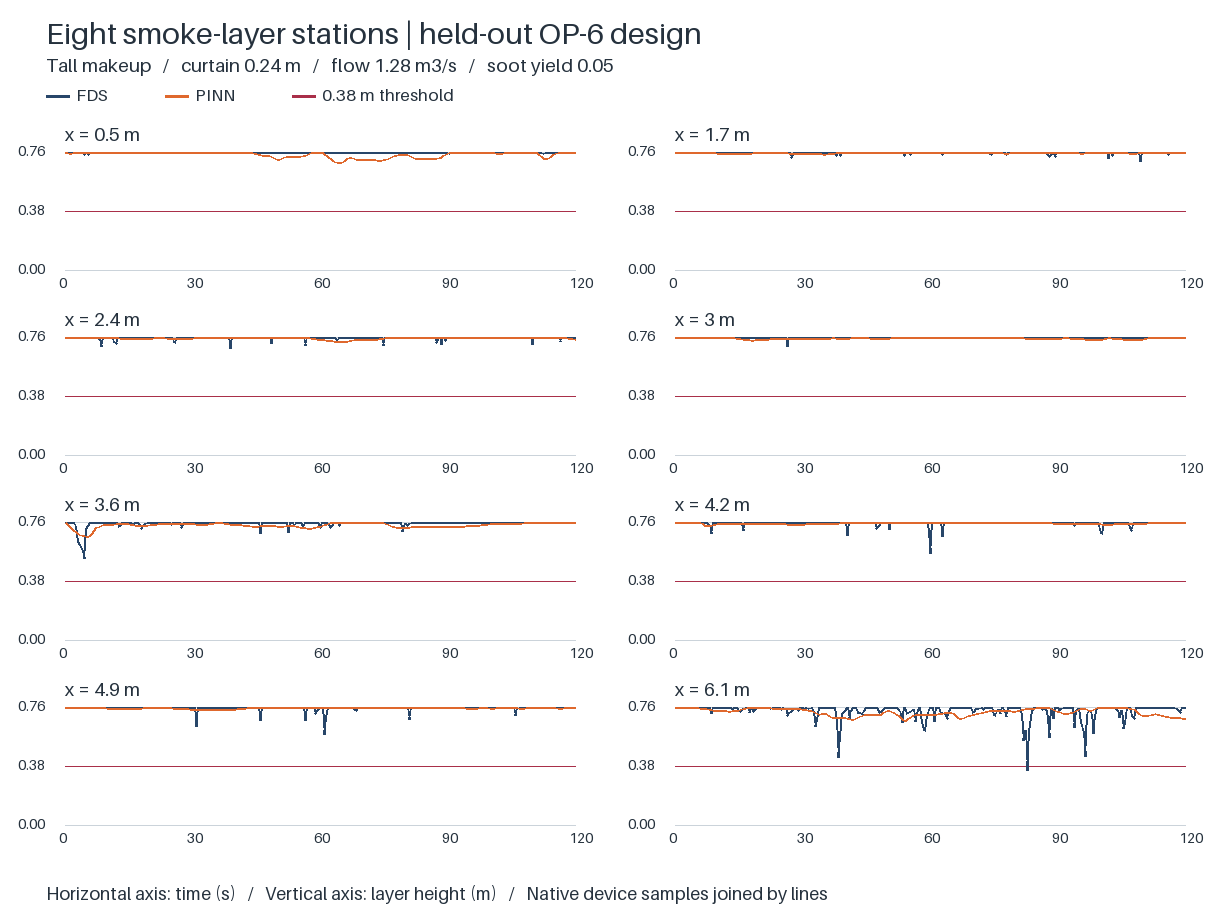
\includegraphics[width=.90\linewidth]{../../09_PINN_Layer/eight_stations.png}}{Figure E1. FDS and PINN thermal layer heights across the eight sampled columns. The far-end station is enlarged in Figure 5.}

\end{document}
